\chapter{Алгоритмы на решетках}
\label{ch:chap2}

В этой главе будут задачи SVP/SIS и LWE, и основанные на них алгоритмы шифрования.

\section{Решетки как математическая структура}
\label{sec:lattice_math}

Решетка -- это периодическая ``сетка'' в пространстве $Z^m$.
Для каждой решетки можно выбрать базис, причем он не единственный.

\begin{figure}[ht]
	\centering
	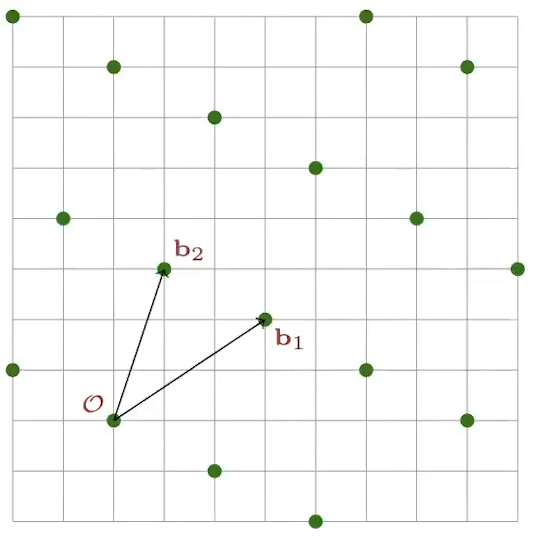
\includegraphics[width=0.5\textwidth]{lattice_basis}
	\caption{Пример решетки и ее базиса при $m = 2$}
	\label{fig:lattice_basis}
\end{figure}

Для них существует некоторый набор ``стандартных'', хорошо изученных задач. Например, GapSVP, SIVP (Shortest Independent Vectors Problem). Эти задачи в сложных случаях (для сложных наборов параметров) не имеют полиномиальных алгоритмов решения.

\section{SVP (Shortest Vector Problem)}

Постановка задачи проста: найти самый короткий вектор $\bm{b_0}$ в решетке $\mathcal{L}$, заданной каким-то базисом.

Сложность задачи растет с размерностью решетки $m$. Обычно рассматриваются приближенные задачи -- поиск вектора с длиной меньше $\gamma \boldsymbol{b_0}$. Имеющиеся алгоритмы (в том числе квантовые) требуют экспоненциальных памяти и времени для задачи с $\gamma = poly(m)$ \cite{svp}.

Квантовые алгоритмы не исправляют ситуацию, поскольку не говорят ничего о геометрических свойствах. Например, алгоритм Шора хорошо справляется с поиском групповой структуры, но не позволяет находить кратчайшие вектора в геометрическом смысле.

\section{SIS (Short Integer Solution)}

Эта задача является алгебраической и на первый взгляд не имеет ничего общего с решетками.

Пусть $\mathds{Z}^n_q$ -- поле векторов размерности $n$ по модулю $q$.
Выберем равномерно случайную матрицу $A \in \mathds{Z}^{n \times m}_q$. Задача -- найти ненулевой $\boldsymbol{z} \in \mathds{Z}^m$ такой, что $A \boldsymbol{z} = \boldsymbol{0} \in \mathds{Z}^n_q$ при условии $\|\boldsymbol{z}\| < \beta \ll q$. 

Если предположить, что SIS сложно решить, то, взяв $m > n \log_2 q$ определим хэш-функцию $f_A: \{0,1\}^m \rightarrow \mathds{Z}^n_q$ как $f_A(\boldsymbol{x}) = A\boldsymbol{x}$. Такая функция будет устойчива к поиску коллизий, поскольку $A\boldsymbol{x} = A \boldsymbol{x'} \Rightarrow A(\boldsymbol{x} - \boldsymbol{x'}) = 0$, то есть $\boldsymbol{z} = \boldsymbol{x} - \boldsymbol{x'} \in \{0, \pm 1\}^m$ -- решение SIS.

\section{Связь SIS и SVP}

Выясним, какое отношение SIS имеет к решеткам.

Матрица $A \in \mathds{Z}^{n \times m}_q$ задает решетку $\mathcal{L^{\perp}} (A) = \{\boldsymbol{z} \in \mathds{Z}^m : A\boldsymbol{z} = \boldsymbol{0}\}$. На Рисунке \ref{fig:lattice_matrix} изображена решетка для случая $m = 2$. Тогда нахождение $\boldsymbol{z}$ для SIS эквивалентно поиску ``короткого'' вектора в решетке $\mathcal{L^{\perp}}(A)$. То есть SIS эквивалентна SVP.

\begin{figure}[ht]
	\centering
	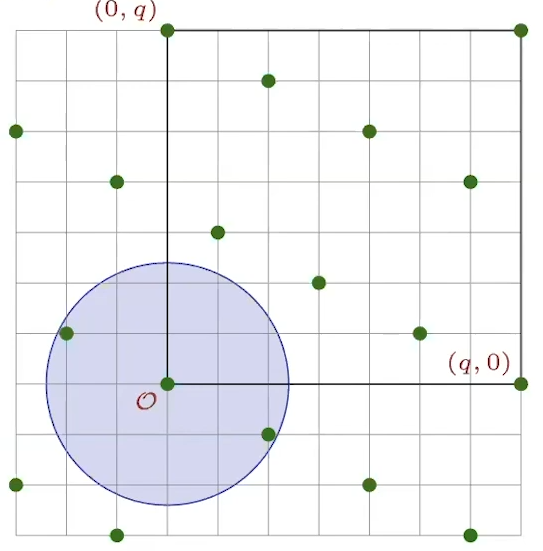
\includegraphics[width=0.5\textwidth]{lattice_matrix}
	\caption{Решетка и ограничение на длину вектора $\boldsymbol{z}$}
	\label{fig:lattice_matrix}
\end{figure}

Важным теоретическим результатом является сведение worst-case (нахождение решения на самых сложных вариантах) к average-case (нахождение решения для случайных вариантов):
Алгоритмом для нахождения ``короткого'' вектора для равномерно случайной $A$ можно решить любую задачу GapSVP и SIVP \cite{Ajtai96}. Поскольку лучшие алгоритмы, которые были найдены, для сложных случаев GapSVP и SIVP -- экспоненциальные, то считается, что полиномиального алгоритма для SIS не существует.

\section{Применение SIS в криптографии}

Предположим, что мы можем сгенерировать равномерно случайную матрицу $A$ с ``секретным ключом'' $T$ (trapdoor). Такой алгоритм существует, почти любая матрица может из равномерного распределения может быть создана в паре с ключом $T$ \cite{short_basis_trapdoor}.
Для подписи мы считаем хэш сообщения $H(\mu)$ и с помощью $T$ находим достаточно короткий $\boldsymbol{z}: A \boldsymbol{z} = H(\mu) \in \mathds{Z}^n_q$.
В качестве $H(\mu)$ можно использовать любую достаточно надежную хэш-функцию (например, SHA).
Для того, чтобы исключить ``обучение'' на выдаваемых $\boldsymbol{z}$ мы будем брать их из дискретного гауссова распределения. Иначе, $T$ может быть восстановлен по набору $\boldsymbol{z}$ для различных $H(\mu)$ \cite{DN12}.

Для создания подписи на другое сообщение $\mu^*$ злоумышленнику требуется найти ``достаточно короткий'' $\boldsymbol{z}$ такой, что $A \boldsymbol{z^*} = H(\mu^*)$. Эта задача и есть SIS.

\section{LWE (Learning With Errors)}

Постановка задачи LWE: необходимо найти секретный $\boldsymbol{s} \in \mathds{Z}^n_q$, зная $\boldsymbol{b}^T = \bm{s}^T A + \bm{e}^T$ -- скалярные произведения случайных векторов с $\boldsymbol{s}$ с некоторой гауссовой ошибкой $\bm{e}$.

Матрица $A$ вновь задает решетку, но уже иначе: $\mathcal{L}(A) = \{ \boldsymbol{z}^T : \boldsymbol{z}^T = \boldsymbol{s}^T A \mod q\}$. Пример приведен на Рисунке \ref{fig:lattice_lwe}. Таким образом, LWE сводится к задаче поиска узла решетки по точке в его окрестности.

\begin{figure}[ht]
	\centering
	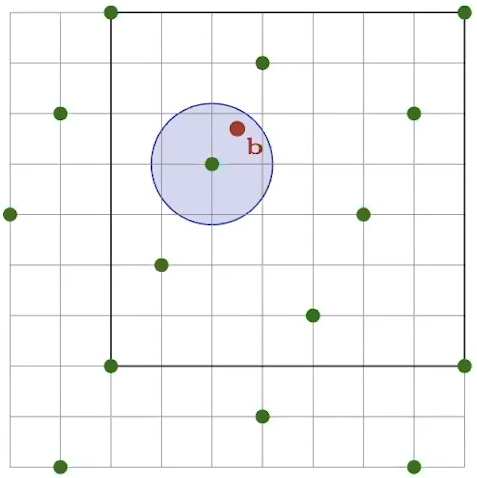
\includegraphics[width=0.5\textwidth]{lattice_lwe}
	\caption{Нахождение узла решетки по точке вблизи него (тут $\bm{e} \notin \mathds{Z}^n_q$ для наглядности)}
	\label{fig:lattice_lwe}
\end{figure}

Теория говорит, что search-LWE -- сложная задача. Есть сведение алгоритма для average-case LWE к worst-case задачам на решетках (GapSVP, SIVP) \cite{Regev05}. Эти задачи считаются не имеющими полиномиального решения даже квантовыми компьютерами, поэтому LWE считается квантово устойчивой.

Более того, можно показать, что если существует алгоритм, отличающий полностью случайные пары $(A, \boldsymbol{b})$ от тех, которые являются скалярным произведением с $\boldsymbol{s}$ (decision-LWE), то его можно свести к алгоритму для search-LWE \cite{Regev05}.

\section{Применение LWE в криптографии}

Агенты А и Б выбирают равномерно случайную матрицу $A \in \mathds{Z}^{n \times n}_q$. Эта матрица будет частью открытого ключа, общего для агентов. После чего агент А выбирает ``короткий'', равномерно случайный вектор $\boldsymbol{s} \in \mathds{Z}^n_q$, Б -- вектор $\boldsymbol{r}$ с такими же свойствами. Агент А вычисляет $\bm{u}^T \approx \bm{r}^T A \in \mathds{Z}^n_q$, агент Б в свою очередь $\bm{v} \approx A \bm{s} \in \mathds{Z}^n_q$. При вычислении $\bm{u}$ и $\bm{v}$ вносится ошибка из гауссова распределения, которое также является заранее выбранным и общеизвестным.

Заметим, что агент А может получить $\bm{r}^T \bm{v} \approx \bm{r}^T A \bm{s} \approx k$. В свою очередь агент Б получает $\bm{u}^T \bm{s} \approx \bm{r}^T A \bm{s} \approx k$. То есть А и Б получили два числа, очень близких к общему числу $k \in \mathds{Z}_q$.

Тогда агент Б может закодировать бит как $c = k + \text{bit} \cdot \frac{q}{2}$.

При дешифровке агент А получает

\begin{equation*}
	c - k \approx \text{bit} \cdot \frac{q}{2} =
	\begin{cases}
		\text{число, близкое к нулю, bit = 0};\\
		\text{число, близкое к } \frac{q}{2} \text{, bit = 1}.
	\end{cases}
\end{equation*}

Для каждого нового бита нужно генерировать новую пару $\bm{s}$, $\bm{r}$, однако существуют способы ослабить это требование.

Рассмотрим задачу со стороны злоумышленника. Он имеет доступ к $\{A, \bm{u}, \bm{v}, c \}$. Его задача -- распознать, $c = k$ или $c = k + \frac{q}{2}$. По сути это -- задача decision-LWE. То есть она считается квантово устойчивой на сегодняшний день. Для злоумышленника набор $\{A, \bm{u}, \bm{v}, c \}$ неотличим от равномерно случайного.

Может показаться, что значения $\bm{r}$ и $\bm{s}$ можно получить обращением матрицы $A$. Однако, попытка применить $A^{-1}$ к $\bm{u}$ или $\bm{v}$ дает
\begin{equation*}
	A^{-1} \bm{u} = A^{-1} A \bm{r} + A^{-1} \bm{e}= \bm{r} + A^{-1} \bm{e}.
\end{equation*}
При этом $A^{-1} \bm{e}$ вносит настолько сильный вклад, что выделить $\bm{r}$ становится невозможным.

\section{Преимущества}

Алгоритмы, основанные на решетках, обладают рядом преимуществ:
\begin{itemize}
	\item задачи на решетках опираются на геометрические свойства, вычисление которых хорошо сопротивляются квантовым атакам;
	\item существуют теоремы, доказывающие, что из worst-case hardness задач следует их average-case hardness;
	\item обладают высокой степенью вычислительного параллелизма за счет линейной структуры.
\end{itemize}

Кроме того, их можно использовать для полностью гомоморфного шифрования (Fully Homomorphic Encryption) -- шифрование, позволяющие совершать математические операции над данными не расшифровывая их.

\endinput